%Gravimetrie-Versuchsbeschreibung
Die Notizen, die während der Messungen gemacht wurden, befinden sich im Anhang in den Abbildungen \ref{fig:mitschrieb1} und \ref{fig:mitschrieb2}

\section{Messung mit dem Gravimeter}

Die Messung mit den beiden vorhandenen Gravimetern wurde auf dem Profil orthogonal zum Basaltgang durchgeführt. Auf dem gleichen Profil wurden schon Messungen mit allen drei der vorherigen Messverfahren durchgeführt. Dies ist in Abbildung \ref{fig:Luisa} zu sehen. Die Lage der Profilpunkte des Gravimetrie-Profils zueinander ist in Skizze \ref{fig:Svenja} zu sehen. Da zwei Gravimeter zur Verfügung standen, wurde mit jedem der Messgeräte jeweils jeder zweite Punkt vermessen. Der Messpunkt G0 in Abbildung \ref{fig:Svenja} bezeichnet den Basispunkt der Messung. Auf
diesem Punkt wurde mit beiden Gravimetern eine Messung durchgeführt. Bei G7 wird das Maximum des Basaltgangs erwartet. Deswegen wurden dort die Messabstände am kleinsten gewählt.

\begin{figure}[!ht]
 \centering
 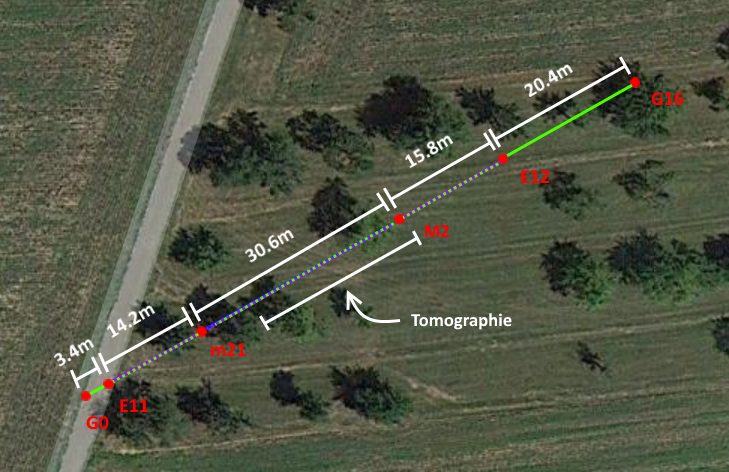
\includegraphics[width=0.6\textwidth]{fig/Luisa}
 \caption[Lage des Profils G0-G16 der Gravimetrie-Messung im Vergleich zu den anderen Profilen]{Lage des Profils G0-G16 der Gravimetrie-Messung im Vergleich zu den anderen Profilen. Die Grafik wurde von Rebekka Kirchgässner und Luisa Rank übernommen.}
 \label{fig:Luisa}
\end{figure}

\begin{figure}[!ht]
 \centering
 \includegraphics[width=\textwidth]{fig/Svenja}
 \caption{ Skizze zur Lage der Profilpunkte des Gravimetrie-Profils}
 \label{fig:Svenja}
\end{figure}

Um die Drift der Messgeräte erfassen und korrigieren zu können, wurden jeweils zwei Messungen auf dem selben Profil im Abstand von mehr als einer Stunde durchgeführt. Dies wurde umgesetzt, indem man mit den Gravimetern einmal das ganze Profil komplett entlang ging und dann mit der zweiten Messung wieder am ersten Messpunkt begann.

Die Messungen wurden mit Gravimetern des Types LaCoste-Romberg(G) durchgeführt. Da Gravimeter sehr empfindliche Messgeräte sind, mussten die Messungen sehr genau und vorsichtig durchgeführt werden. Das Messgerät hat eine 
theoretische Auflösung von 0,01\,mGal.

Um einen Messpunkt zu vermessen, wurde das Gravimeter zunächst neben den mit zwei Pflöcken markierten Punkt gestellt. Mit Hilfe zweier Libellen wurde es horizontal ausgerichtet. Einer der beiden Pflöcke 
war bis auf eine Handbreite in den Boden geschlagen und diente zur exakten Messung der Instrumentenhöhe. Diese Höhe muss bis auf 5\,mm genau bestimmt werden, um die Korrektur der Instrumentenhöhe so durchführen zu können, dass sie nicht das Ergebnis verfälscht.
Wenn das Gravimeter nicht mehr bewegt wurde, konnte die Arretierung gelöst werden. Solange die Messung durchgeführt wurde, achtete man darauf, dass sich keine Person dem Messgerät näherte oder sich die Personen in der Nähe stark bewegten. Dies war wichtig, da es einen sofort sichtbaren Einfluss auf die Messung hatte, wenn sich eine Person näherte.

Die Messung wurde immer zu dritt durchgeführt. Eine Person war verantwortlich für einen Sonnenschirm, der über das Messgerät gehalten wurde, eine für das Ablesen der Messwerte 
und eine dritte Person führte das Messprotokoll. Im Messprotokoll (siehe Abbildungen \ref{fig:MP1_156} bis \ref{fig:MP2_686} im Anhang) wurde die Instrumentenhöhe und die Zeit direkt mit aufgeschrieben, um noch vor Ort die Instrumentenhöhenkorrektur nach Gleichung \eqref{eq:Freiluft} und die Gezeitenkorrektur mit einem Diagramm durchzuführen.
% Dieses befindet sich im Anhang in Abbildung ???.
Es ist hilfreich, diese Korrekturen direkt vor Ort durchzuführen, um die Messungen der verschiedenen Geräte, die zu unterschiedlichen Zeiten durchgeführt wurden, vergleichen zu können und schon im Feld feststellen zu können, ob die Daten auswertbar werden oder es zu zu großen Messunsicherheiten kam.

\section{Tachymetrie}

Mit einem elektronischen Tachymeter TC 500 wurde die Lage und Höhe der Messpunkte, die mit den Gravimetern vermessen wurden, relativ zu einem Basispunkt bestimmt. Dazu wurde der Reflektor an dem zu vermessenden Punkt aufgestellt und mit dem sehr genau horizontierten Messgerät angepeilt. Mit einem Laser wurde die Entfernung gemessen. Durch eine Interne Winkelmessung kann der Rechts- und Hochwert bestimmt werden, der für die geologische Reduktion benötigt wird. Die Messprotokolle zu diesem Versuchsteil sind im Anhang unter Abbildung \ref{fig:MPTachymetrie1} und \ref{fig:MPTachymetrie2} zu finden.

\section{Vermessung mit GPS}

Mit einem GPS-Gerät wurden die Pflöcke, mit denen alle Profil-Punkte und sonstigen wichtigen Orte während der Messungen markiert wurden, eingemessen. Es wurden die GPS-Koordinaten, die Zeit der Messung und die Art der Lösung des Gleichungssystems gespeichert. Manchmal hatte das Messgerät durch zum Beispiel Bäume keinen Kontakt zu genug Satelliten, sodass die Lage der Punkte nicht so genau wie sonst bestimmt werden konnte.

Bei der Messung selbst musste darauf geachtet werden, dass die Stange an der das Gerät befestigt war, mit zwei Stangen möglichst genau vertikal ausgerichtet wurde. Zur Kontrolle der Ausrichtung diente eine Punkt-Libelle. Außerdem musste ihre Länge notiert werden, um auf die Koordinaten auf Boden-Niveau schließen zu können. Nach einer Messung konnten der vermessene Punkt im Gerät umbenannt werden, um die Übersichtlichkeit zu gewährleisten. Hier machte sich bemerkbar, wie hilfreich unsere während der Versuchstage angefertigte Karte der Profilpunkte war. Außerdem stellte sich unsere Beschriftung der Pflöcke als sehr hilfreich und strukturiert heraus.